\documentclass[journal]{IEEEtran}
\usepackage{amsmath,amssymb,amsfonts}
\usepackage{algorithmic}
\usepackage{algorithm}
\usepackage{graphicx}
\usepackage{textcomp}
\usepackage{xcolor}
\usepackage{booktabs}
\usepackage{array}
\usepackage{multirow}
\usepackage{balance}
\usepackage{hyperref}
\usepackage{bm}
\usepackage{epstopdf}
\usepackage[caption=false,font=footnotesize]{subfig}
\usepackage{tikz}
\usepackage{cite}

% Revision marker: wrap text added or rewritten in this revision in \new{...}
% to display in blue for the prof's review pass. Remove the macro body
% (replace with just \def\new#1{#1}) to switch off the highlighting.
\newcommand{\new}[1]{#1}
% Section IV-E rewrite marker (2026-05-03). Removable: replace body with #1.
\newcommand{\revIVE}[1]{#1}
% Round-2 revision marker (TAI-2026-May-A-00956). Marked build sets this to blue.
\newcommand{\rev}[1]{#1}
\usetikzlibrary{positioning,shapes.geometric,arrows.meta,fit,backgrounds,calc}


\begin{document}

\title{SCOPE-FD: A Client Selection Method in Federated Distillation for Massive-MIMO Systems}

\author{
% Authors to be added
}

\maketitle

\begin{abstract}
\rev{Federated distillation lets edge devices train a shared model by exchanging only their predictions on a public dataset. That costs far less over a wireless link than sending weights. A base station can serve only a few of its devices per round, so it must choose which ones. Client selection is well studied for federated learning, where devices are ranked by a utility signal such as local loss. Federated distillation averages predictions rather than weights. That flattens the per-device signals, so the same rules do not carry over. Published systems for massive multiple-input multiple-output networks avoid the question by assuming that every device participates in every round. This paper proposes Server-aware Coverage with Over-round Participation Equalization, or SCOPE-FD, a deterministic selector for partial participation. It rotates devices by how far each has fallen behind a uniform participation target. Ties go to devices holding classes the server predicts poorly. The participation imbalance this produces is not merely bounded but exact. It follows from the pool size, the number served per round and the training horizon. An operator can therefore compute it before training starts. Composing that guarantee with the convergence bound of the underlying framework gives a rate in communication rounds. The rate holds for every device rather than on average. Accuracy holds level with uniform random selection and leads it where participation is sparsest. Participation fairness is therefore constructible rather than merely achievable. It becomes something an operator can commit to in advance rather than verify afterwards.}
\end{abstract}

\begin{IEEEkeywords}
Federated distillation, client selection, massive MIMO, participation fairness, knowledge distillation, communication efficiency.
\end{IEEEkeywords}

{\renewcommand{\abstractname}{Impact Statement}
\begin{abstract}
\rev{Wireless networks are starting to train shared artificial intelligence models across phones, wearables and vehicles. The data never leaves the device. Only a handful of devices can be served in each training round. Picking them at random means some devices contribute far more than others. Whose data shapes the model then becomes partly a matter of chance. This work replaces that lottery with a rotation. Its fairness follows from three quantities a network operator already knows. It can therefore be stated before a deployment is switched on rather than measured after it has run. Operators give up no accuracy in exchange. Artificial intelligence systems face a growing legal duty to evidence fair treatment of the people they serve. Committing to a participation guarantee in advance, rather than reporting one in hindsight, changes what a deployment can promise its users and its regulators.}
\end{abstract}}
\vspace{-1em}
\section{Introduction}
\label{sec:introduction}
\IEEEPARstart{F}{EDERATED} Learning (FL) \cite{mcmahan2017communication}, \cite{borazjani2026redefining} lets a population of devices train a shared model under a central server without their data ever leaving them \cite{rao2025privacy, huang2024survey}. In each round the selected clients train locally and upload the updated model parameters for aggregation. Uploading full model weights does not scale to modern architectures over a wireless edge, particularly when many devices share the same connectivity. Federated Distillation (FD) \cite{jeong2018communication} avoids that cost by having each client upload only its output logits on a shared public dataset \cite{itahara2023distillation}. Such a logit-only exchange cuts the per-round communication overhead substantially and lets clients train heterogeneous local architectures \cite{sattler2022cfd, sattler2023fedaux, chan2021fedhe, cho2023clustered, wu2024fedict}.

The integration of FD with massive multiple-input multiple-output (mMIMO) wireless backbones is investigated in \cite{mu2024fedtskd}, where channel hardening and zero-forcing precoding handle the noisy uplink and downlink. The FedTSKD framework proposed there establishes a dynamic training schedule, an $\mathcal{O}(1/t)$ convergence bound, and a channel-aware aggregation rule for FD over mMIMO. It specializes the earlier wireless-FD line \cite{ahn2019wireless} and the broader wireless FL over fading channels work \cite{amiri2020federated, vu2020cell}.

That work assumes full client participation, so all $N$ clients transmit logits in every round, and the assumption is uniformly adopted across the FD literature \cite{itahara2023distillation, sattler2022cfd, sattler2023fedaux, wu2024fedict}. It breaks down whenever a deployment holds more devices than the scheduler can admit, runs under a per-round energy budget \rev{\cite{thakur2026grace}}, or shares a contention-limited uplink. Each case forces the system to admit only $K \ll N$ clients per round. \new{In FL, the question of which $K$ out of $N$ clients to admit per round has been studied from several directions, including resource-aware, importance- and channel-aware, bandit-driven, and submodular formulations \cite{nishio2019client, yang2020scheduling, ren2020scheduling, shi2020joint, xia2020mab, cho2020bandit, balakrishnan2022divfl}, as reviewed in Section~\ref{ssec:rw-fl-selection}.} In FD the client selection problem has received scant attention. The closest prior work is the active data sampling method of \cite{liu2022active}, which selects public-dataset samples to distill on rather than clients to admit.

None of those FL selectors is designed for FD, for a structural reason. The FD aggregation rule is data-size-weighted logit averaging \cite{mu2024fedtskd, itahara2023distillation}, which flattens per-client quality differences once the selected set is fixed. The composition of that set, rather than any intra-client quality gradient, therefore drives the server model. FL behaves differently, since each local gradient enters the aggregate directly and ranking clients by training loss \cite{cho2020bandit, xia2020mab} or gradient norm \cite{wang2019adaptive} produces a meaningful aggregate signal. The right question in FD client selection is therefore not how to score individual clients along a single utility axis. It is how to use every client's data uniformly across rounds, while nudging the within-round composition towards the regions of the label space where the server is currently uncertain.

\subsection{Contributions}
\label{ssec:contributions}

This paper proposes SCOPE-FD (Server-aware Coverage with Over-round Participation Equalization), a deterministic client selector for FD over mMIMO networks, built on the FedTSKD substrate of \cite{mu2024fedtskd}. Existing FL selectors \cite{nishio2019client, cho2020bandit, xia2020mab, balakrishnan2022divfl} score clients by utility or by coverage but not both, while existing FD work \cite{mu2024fedtskd, itahara2023distillation, liu2022active} either assumes full participation or addresses it only along the data-sampling direction. The proposed score instead composes participation balance, server-side class under-prediction and per-round class coverage \revIVE{with non-negative coefficients held fixed across all configurations}. To the best of the authors' knowledge it is the first deterministic fairness-guaranteed selector tailored to the data-size-weighted logit-averaging rule of FD under partial participation. The main contributions follow.

\begin{enumerate}
    \item \textit{Three-Term Deterministic Selector for FD.} We design a selector combining a participation-debt rotation term, a server-side under-prediction bonus and a class-coverage penalty, with the debt term primary and the other two breaking ties inside debt-equal cohorts. It carries zero trainable parameters, unlike the reinforcement-learning and neural-bandit FL selectors \rev{\cite{kazemi2026robust, xia2020mab}} that maintain $\mathcal{O}(N\cdot K)$ trainable states, and fills $K$ slots in $\mathcal{O}(KNC)$ time per round for $C$ label classes.

    \item \textit{Participation-Fairness Guarantee.} We prove that the per-client cumulative participation counts differ by at most one at every round. When $K$ divides $N$ this sharpens to exact equality at the end of every $\lceil N/K \rceil$-round cycle. \rev{We further show that the cumulative coefficient after $R$ rounds is not merely bounded but exactly $m(N-m)/(NKR)$, with $m = KR \bmod N$. This makes the $\mathcal{O}(1/R)$ bound tight and identifies $N \mid KR$ as the exact condition for it to vanish, so the fairness of a deployment can be computed in advance.}

    \item \textit{\rev{Round-Indexed Convergence under Partial Participation.}} The selector modifies only the composition of the per-round subset, leaving the local training, distillation and aggregation steps of FedTSKD \cite{mu2024fedtskd} unchanged. \rev{Composing the per-client bound of \cite{mu2024fedtskd} with the participation guarantee gives a rate of $\mathcal{O}(N/(KR))$ in communication rounds that holds for every client at every finite horizon rather than on average. It asks for nothing beyond the assumptions of \cite{mu2024fedtskd}, which we work through one at a time, and returns their $\mathcal{O}(1/R)$ result at full participation.}

    \item \textit{Experimental Analysis.} \rev{Every quantity is a mean with a standard deviation over independent seeds. The datasets are Fashion-MNIST with non-independent and identically distributed (non-IID) Dirichlet partitions, MNIST and a spoken-digit corpus. The sweeps cover the cohort size $K$, the Dirichlet concentration $\alpha$, the downlink signal-to-noise ratio (SNR), the pool size $N$ and the two coefficients. The selector lowers the participation Gini coefficient by roughly an order of magnitude against uniform random in every configuration tested. On accuracy it leads where participation is sparse, ties at the headline setting and trails once the cohort reaches twenty clients. A four-way ablation separates each score term and four published selectors ported into FD serve as comparison points.}
\end{enumerate}

%The proposed method is positioned as a fairness-first selector for FD; head-to-head comparison against utility-driven FL selectors adapted to FD is left to future work.

\textit{Organization.} The rest of this paper is organized as follows. Section~\ref{sec:related-work} provides background on client selection in FL and FD. Section~\ref{sec:system-model} details the system model and the FD aggregation rule under partial participation. The proposed SCOPE-FD algorithm is described in Section~\ref{sec:scope-alg}, followed by the theoretical analysis in Section~\ref{sec:theory}. Experimental results are presented in Section~\ref{sec:experiments}, and finally Section~\ref{sec:conclusion} concludes this paper.

% ============================================================================
% SECTION II: RELATED WORK
% ============================================================================
\section{Background}
\label{sec:related-work}

\subsection{Client Selection in Federated Learning}
\label{ssec:rw-fl-selection}

Existing FL client-selection work spans several directions. Resource-aware methods such as FedCS \cite{nishio2019client} admit the maximum number of clients that can train and upload within a per-round deadline. Importance- and channel-aware scheduling \cite{yang2020scheduling, ren2020scheduling, shi2020joint} jointly incorporates wireless link state and gradient magnitude into a per-client priority score. Bandit-driven online selectors \cite{xia2020mab}, \cite{cho2020bandit} treat per-client utility as the unknown reward of a multi-armed bandit. DivFL \cite{balakrishnan2022divfl} constructs the per-round client subset by greedily maximizing a submodular function over client gradients. Complementary lines include adaptive resource-constrained selection \cite{wang2019adaptive} and the $q$-fair fairness objective \cite{li2020qffl}. \rev{Fairness has more recently been made the selection criterion itself rather than a constraint on it, as in the inclusive selection framework of \cite{arisdakessian2026vox}, which scores clients on participation equity alongside utility. That line shares the objective of the present work, but it is formulated for FedAvg, where the selection signal enters the parameter average directly.}

In all of the above the aggregation rule is FedAvg \cite{mcmahan2017communication}, where each selected update enters the aggregate directly, which is what makes a per-client quality score meaningful at the server. That property does not survive the FD aggregation rule.

\rev{Four of these selectors serve as comparison points in Section~\ref{sec:experiments}, each ported into the FD pipeline. A client in FD uploads no gradient, so any selector whose native signal is a model update needs a substitute that FD produces. Two are available, namely the static label histogram and the per-round logit vector on the public set. DivFL \cite{balakrishnan2022divfl} performs facility-location submodular maximization over client gradients and is ported by replacing the gradient with the public-set logit vector, which preserves the greedy procedure and changes only the representation. SubTrunc \cite{castillo2024subtrunc} performs truncated submodular maximization diversified by client loss and ports directly, since that loss is already computed every round. UnionFL \cite{castillo2024unionfl} diversifies by historical participation, which maps onto the counts the selector already maintains. Oort \cite{lai2021oort} is a utility-based FL selector run without modification, which measures directly what happens when an FL rule is transferred to FD unchanged.}

\subsection{Federated Distillation Algorithms and Wireless Physical Layer Integration}
\label{ssec:rw-fd}

The FD paradigm originates in \cite{jeong2018communication}, which proposed using knowledge distillation \cite{hinton2015distilling} to communicate model outputs rather than parameters. The semi-supervised variant DS-FL follows in \cite{itahara2023distillation}, where a shared unlabeled public dataset carries the logit exchange and the server aggregates per-client logits by data-size-weighted averaging. Communication-efficient logit transmission has been further investigated in \cite{sattler2022cfd}, where a soft-label quantization and delta-coding scheme is proposed, and in \cite{sattler2023fedaux}, where unlabeled auxiliary data is exploited through a certainty-weighted ensemble. The model-heterogeneous variant FedHe is introduced in \cite{chan2021fedhe}, the clustered knowledge-transfer scheme of \cite{cho2023clustered} extends FD to the personalization setting, and the multi-task formulation FedICT in \cite{wu2024fedict} addresses multi-access edge computing scenarios.

Wireless-channel-aware FD is initiated in \cite{ahn2019wireless} for distributed edge learning over fading uplinks, and later extended to cooperative learning where the channel fading is accounted for on both the uplink and the downlink. The integration of FD with mMIMO backbones is then carried out in \cite{mu2024fedtskd}, where the FedTSKD framework is proposed together with its $\mathcal{O}(1/t)$ convergence guarantee. The FedTSKD work specializes the broader wireless FL over fading channels line of research \cite{amiri2020federated, vu2020cell} to the FD paradigm. There the noise tolerance of the logit layer interacts favorably with the channel hardening property of mMIMO, and zero-forcing precoding nulls out the inter-user interference.

All of the FD works above aggregate by data-size-weighted logit averaging, so once the per-round subset is fixed each client's contribution is governed only by its data-size weight and within-round scoring carries far less effect than in FL. None of them addresses how that subset should be constructed when only a strict subset can be admitted, since full participation is uniformly assumed.

\subsection{Client Selection in Federated Distillation}
\label{ssec:rw-fd-selection}

The closest prior work is the active data sampling method of \cite{liu2022active}, which adaptively selects the public-dataset samples to distill on. That is orthogonal to client selection, since the rule operates on public samples rather than on the client population. Fairness-aware FL formulations such as the $q$-fair objective of \cite{li2020qffl} are a relevant baseline, but their constraint is defined on the FedAvg rule and does not transfer to logit averaging without modification.

No existing work addresses these three concerns together. They are partial participation in FD, the effect of data-size-weighted logit averaging on how the per-round subset shapes the server model, and the wireless-channel impairments of an mMIMO backhaul. The proposed SCOPE-FD algorithm is designed to address all three together, while preserving the convergence guarantee of FedTSKD \cite{mu2024fedtskd}.

\textit{Remark (Delta to \cite{mu2024fedtskd}).} The FedTSKD framework of \cite{mu2024fedtskd}, developed by the present authors' research group,\footnote{FedTSKD \cite{mu2024fedtskd} is from the same research group as the present work and is treated here as an off-the-shelf substrate.} supplies the FD-over-mMIMO substrate. That substrate is the dynamic local-training schedule, the zero-forcing uplink and downlink processing, the data-size-weighted logit-averaging aggregation rule and the $\mathcal{O}(1/t)$ convergence analysis. SCOPE-FD inherits all of it without modification. What is new here is the partial-participation client-selection problem itself, which \cite{mu2024fedtskd} does not address. The remaining contributions are the deterministic three-term score with non-negative coefficients held fixed across configurations, the participation Gini guarantee of Section~\ref{ssec:participation-balance}, and \rev{the round-indexed convergence corollaries of Section~\ref{ssec:convergence-compat}.}

% ============================================================================
% SECTION III: SYSTEM MODEL AND PROBLEM FORMULATION
% ============================================================================
\section{System Model and Problem Formulation}
\label{sec:system-model}

\begin{figure*}[!t]
\centering
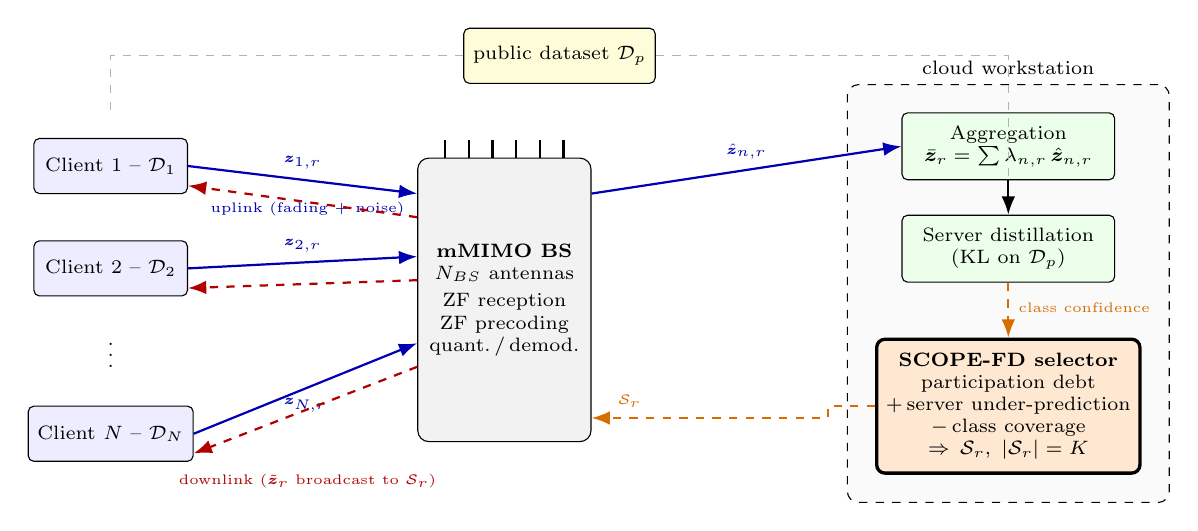
\begin{tikzpicture}[
    font=\footnotesize, >=Latex,
    client/.style  ={draw, rounded corners=2pt, minimum height=0.7cm, minimum width=1.95cm, align=center, fill=blue!7,    font=\scriptsize},
    block/.style   ={draw, rounded corners=2pt, minimum height=0.85cm,minimum width=2.7cm, align=center, fill=green!8,   font=\scriptsize},
    scopebox/.style={draw, rounded corners=3pt, minimum height=1.7cm, minimum width=3.2cm, align=center, fill=orange!18, very thick, font=\scriptsize},
    bs/.style      ={draw, rounded corners=4pt, minimum height=3.6cm, minimum width=2.2cm, align=center, fill=gray!10,   font=\scriptsize},
    pub/.style     ={draw, rounded corners=2pt, minimum height=0.7cm, minimum width=2.3cm, align=center, fill=yellow!15, font=\scriptsize}
]

% --- Clients ---
\node[client] (c1) at (0,  2.6) {Client $1$ -- $\mathcal{D}_1$};
\node[client] (c2) at (0,  1.3) {Client $2$ -- $\mathcal{D}_2$};
\node[font=\scriptsize] at (0, 0.3) {$\vdots$};
\node[client] (cn) at (0, -0.8) {Client $N$ -- $\mathcal{D}_N$};

% --- mMIMO BS ---
\node[bs] (bs) at (5.0, 0.9) {\textbf{mMIMO BS}\\$N_{BS}$ antennas\\[2pt]ZF reception\\ZF precoding\\quant.\,/\,demod.};
\foreach \x in {-0.75,-0.45,-0.15,0.15,0.45,0.75}
  \draw[thick] ($(bs.north)+(\x,0)$) -- ++(0, 0.22);

% --- Public dataset ---
\node[pub] (pub) at (5.7, 4.0) {public dataset $\mathcal{D}_p$};

% --- Cloud workstation contents ---
\node[block] (agg)  at (11.4,  2.85) {Aggregation\\$\bar{\bm{z}}_r=\sum\lambda_{n,r}\,\hat{\bm{z}}_{n,r}$};
\node[block] (dist) at (11.4,  1.55) {Server distillation\\(KL on $\mathcal{D}_p$)};
\node[scopebox] (sel) at (11.4, -0.45) {\textbf{SCOPE-FD selector}\\participation debt\\$+\,$server under-prediction\\$-\,$class coverage\\$\Rightarrow\,\mathcal{S}_r,\;|\mathcal{S}_r|=K$};

% --- Cloud bounding box ---
\begin{scope}[on background layer]
  \node[draw, dashed, rounded corners=4pt, fit=(agg)(dist)(sel), inner sep=10pt, fill=gray!4,
        label={[font=\scriptsize]above:cloud workstation}] (cloud) {};
\end{scope}

% --- UL arrows: clients -> BS (solid blue) ---
\draw[->, thick, blue!70!black] (c1.east) -- node[midway, above, font=\tiny]{$\bm{z}_{1,r}$} ($(bs.west)+(0, 1.35)$);
\draw[->, thick, blue!70!black] (c2.east) -- node[midway, above, font=\tiny]{$\bm{z}_{2,r}$} ($(bs.west)+(0, 0.55)$);
\draw[->, thick, blue!70!black] (cn.east) -- node[midway, below, font=\tiny]{$\bm{z}_{N,r}$} ($(bs.west)+(0,-0.55)$);
\node[font=\tiny, blue!70!black] at (2.5, 2.05) {uplink (fading + noise)};

% --- DL arrows: BS -> clients (dashed red) ---
\draw[->, thick, red!70!black, dashed] ($(bs.west)+(0, 1.05)$) -- ($(c1.east)+(0,-0.25)$);
\draw[->, thick, red!70!black, dashed] ($(bs.west)+(0, 0.25)$) -- ($(c2.east)+(0,-0.25)$);
\draw[->, thick, red!70!black, dashed] ($(bs.west)+(0,-0.85)$) -- ($(cn.east)+(0,-0.25)$);
\node[font=\tiny, red!70!black] at (2.5, -1.4) {downlink ($\tilde{\bm{z}}_r$ broadcast to $\mathcal{S}_r$)};

% --- BS -> Aggregation (recovered logits) ---
\draw[->, thick, blue!70!black] ($(bs.east)+(0, 1.35)$) -- node[midway, above, font=\tiny]{$\hat{\bm{z}}_{n,r}$} (agg.west);

% --- Aggregation -> Distillation ---
\draw[->, thick] (agg.south) -- (dist.north);

% --- Distillation -> SCOPE selector (feedback) ---
\draw[->, thick, orange!85!black, dashed] (dist.south) -- node[right, font=\tiny, pos=0.45]{class confidence} (sel.north);

% --- SCOPE selector -> BS (scheduling decision) ---
\draw[->, thick, orange!85!black, dashed]
   (sel.west) -- ++(-0.6,0) |- ($(bs.east)+(0,-1.5)$)
   node[font=\tiny, pos=0.92, above]{$\mathcal{S}_r$};

% --- Public dataset connections (thin grey, dashed) ---
\draw[dashed, gray!60] (pub.west) -| ($(c1.north)+(0, 0.3)$);
\draw[dashed, gray!60] (pub.east) -| ($(dist.north)+(0, 0.4)$);

\end{tikzpicture}
\caption{Architecture of SCOPE-FD over an mMIMO backbone. Here $\bm{z}_{n,r}$, $\hat{\bm{z}}_{n,r}$ and $\tilde{\bm{z}}_r$ are the uplink logits, the ZF-equalized logits at the BS and the post-distillation logits broadcast downlink. The cloud workstation sits with the BS over a wired link and hosts the server model, the distillation step and the selector, so the only over-the-air segment is the BS-to-client interface. Solid blue arrows are uplink streams, dashed red the downlink broadcast and dashed orange the control path returning $\mathcal{S}_r$.}
\label{fig:system_model}
\end{figure*}

\subsection{Federated Distillation Setup}
\label{ssec:fd-setup}

Consider an FD system where a base station (BS) equipped with $N_{BS}$ antennas serves $N$ single-antenna clients over an mMIMO wireless backbone. Client $n$ holds a private local dataset $\mathcal{D}_n = \{(\bm{x}_i, y_i)\}_{i=1}^{|\mathcal{D}_n|}$, where $\bm{x}_i$ is the input sample and $y_i \in \{1, \dots, C\}$ its class label, and no local dataset is shared with the BS at any stage. To capture the heterogeneity of edge deployments, the per-class proportions on each client are drawn from a Dirichlet distribution $\text{Dir}(\alpha)$ over the label space \cite{hsu2019measuring}, with smaller $\alpha$ giving more skewed partitions. A public unlabeled dataset $\mathcal{D}_p = \{\bm{x}_p\}_{p=1}^{|\mathcal{D}_p|}$ shared by the BS and all clients carries the per-client logit exchange \cite{itahara2023distillation}. Since only logits are transmitted, the clients are free to adopt heterogeneous local architectures \cite{chan2021fedhe}.

The local loss at client $n$ is given by
\begin{equation}
L_n(\bm{w}_n) = \frac{1}{|\mathcal{D}_n|} \sum_{(\bm{x}_i, y_i) \in \mathcal{D}_n} \ell(\bm{w}_n; \bm{x}_i, y_i),
\label{eq:local_loss}
\end{equation}
where $\bm{w}_n$ denotes the local model parameters and $\ell(\cdot)$ is the per-sample cross-entropy. The server-side objective is to minimize the data-size-weighted sum of the local losses, namely
\begin{equation}
\min_{\{\bm{w}_n\}} \; F\!\left(\{\bm{w}_n\}\right) = \sum_{n=1}^{N} \frac{|\mathcal{D}_n|}{|\mathcal{D}|} L_n(\bm{w}_n),
\label{eq:global_obj}
\end{equation}
where $|\mathcal{D}| = \sum_{n=1}^{N} |\mathcal{D}_n|$. Following \cite{mu2024fedtskd}, each communication round $r$ consists of three stages, viz., local training, uplink communication and server-side aggregation, and downlink broadcast and local distillation. The overall architecture, including the proposed selector at the cloud workstation, is summarized in Fig.~\ref{fig:system_model}.

In the local training stage, every client $n \in \mathcal{S}_r$ runs $E_r$ steps of stochastic gradient descent (SGD) on its private dataset, where $\mathcal{S}_r$ denotes the set of clients selected in round $r$. \rev{The schedule $E_r$ is set by the training configuration and never by the selector. It is held constant across rounds in every experiment reported here.} The updated local parameters are then used to compute the per-sample logits $\bm{z}_{n,r}$ on the public dataset $\mathcal{D}_p$. After quantization and modulation, the logits are uploaded to the BS through the mMIMO uplink, and the received signal at the BS can be written as
\begin{equation}
\bm{Y}^{(\text{UL})}_{r} = \sum_{n \in \mathcal{S}_r} \bm{H}_{n,r} \bm{Z}_{n,r}^{T} \sqrt{\frac{P_{\text{UL}}}{N_D \sigma_z^2}} + \bm{\Omega}^{(\text{UL})}_{r},
\label{eq:ul_signal}
\end{equation}
where $\bm{Y}^{(\text{UL})}_{r} \in \mathbb{C}^{N_{BS} \times N_D}$ stacks the $N_D$ received symbol periods column-wise, $\bm{H}_{n,r} \in \mathbb{C}^{N_{BS} \times 1}$ is the uplink channel column vector between the single-antenna client $n$ and the $N_{BS}$-antenna BS, $\bm{Z}_{n,r} \in \mathbb{C}^{N_D \times 1}$ is the complex-valued symbol representation of $\bm{z}_{n,r}$ obtained after quantization and modulation, so that $\bm{H}_{n,r}\bm{Z}_{n,r}^{T}$ is the rank-one $N_{BS}\times N_D$ matrix received from client $n$, $P_{\text{UL}}$ is the uplink transmit power in linear scale, $N_D$ is the number of complex data streams per logit vector, $\sigma_z^2$ is the per-symbol average power normalization in linear scale, and $\bm{\Omega}^{(\text{UL})}_{r}$ is the receiver-side complex Gaussian noise. The scaling factor in (\ref{eq:ul_signal}) splits $P_{\text{UL}}$ uniformly across the $N_D$ streams and normalizes each entry of $\bm{Z}_{n,r}$ to unit average power. With zero-forcing (ZF) reception, the per-client logits at the BS can be recovered as
\begin{equation}
\hat{\bm{z}}_{n,r} = \bm{z}_{n,r} + \bm{\omega}^{(\text{UL})}_{n,r},
\label{eq:ul_zf}
\end{equation}
where the variance of the post-equalization noise $\bm{\omega}^{(\text{UL})}_{n,r}$ is suppressed by a factor proportional to $N_{BS}$, owing to the channel hardening property of the mMIMO array \cite{mu2024fedtskd}, \cite{vu2020cell}. \rev{Recovering the $K$ per-client streams by ZF requires the composite uplink channel formed by stacking $\{\bm{H}_{n,r}\}_{n \in \mathcal{S}_r}$ column-wise, an element of $\mathbb{C}^{N_{BS} \times K}$, to have full column rank, so the cohort size is bounded by the array, $K \le N_{BS}$. The per-round budget is therefore set by the spatial dimensions the BS can separate rather than by the size of the client pool.}

\subsection{FD Aggregation under Partial Participation}
\label{ssec:fd-aggregation}

After dequantization and demodulation at the BS, the round-$r$ aggregated logit is formed by data-size-weighted averaging over the selected clients, that is,
\begin{equation}
\bar{\bm{z}}_r = \sum_{n \in \mathcal{S}_r} \lambda_{n,r} \, \hat{\bm{z}}_{n,r}, \quad \lambda_{n,r} = \frac{|\mathcal{D}_n|}{\sum_{j \in \mathcal{S}_r} |\mathcal{D}_j|}.
\label{eq:agg}
\end{equation}
The server-model parameters are then updated through a distillation step that minimizes the Kullback-Leibler divergence between the server-model output and $\bar{\bm{z}}_r$ on the public dataset \cite{hinton2015distilling}. The post-distillation logits are subsequently quantized, modulated, precoded with a zero-forcing precoder, and broadcast to the selected clients over the mMIMO downlink. Each selected client then performs a local distillation step that updates its local model. As in the uplink, the downlink post-equalization noise variance is suppressed by the channel hardening of the mMIMO array \cite{mu2024fedtskd}.

Once $\mathcal{S}_r$ is fixed, $\bar{\bm{z}}_r$ depends on the per-client logits only through the weights $\lambda_{n,r}$, so the over-round composition of $\mathcal{S}_r$ rather than any within-round utility drives the server model, which is what the proposed selector shapes.

\subsection{Participation Fairness and Problem Statement}
\label{ssec:problem-statement}

To quantify the per-client participation fairness, the Gini coefficient over the cumulative participation counts is adopted. After $R$ rounds, let $n_i^{(R)}$ denote the total number of rounds in which client $i$ has been selected. The participation Gini coefficient is given by
\begin{equation}
G^{(R)} = \frac{\sum_{i,j} \left|n_i^{(R)} - n_j^{(R)}\right|}{2N \sum_{i=1}^{N} n_i^{(R)}}.
\label{eq:gini}
\end{equation}
A perfectly balanced selection policy yields $G^{(R)} = 0$, whereas uniform random selection yields $G^{(R)} > 0$, with the imbalance growing as the participation ratio $K/N$ shrinks.

The goal of this work is to design a selection policy $\pi$ that returns $\mathcal{S}_r \subset \{1, \dots, N\}$ with $|\mathcal{S}_r| = K$ in each round $r$, so as to minimize the FD convergence error while keeping the participation Gini coefficient small. Letting $\{\bm{w}_n^{(R)}\}$ denote the local model parameters after $R$ rounds under policy $\pi$, the problem can be formulated as
\begin{equation}
\min_{\pi} \; \mathbb{E}\!\left[F\!\left(\{\bm{w}_n^{(R)}\}\right)\right] - F^{*},
\label{eq:problem}
\end{equation}
subject to three constraints. First, $|\mathcal{S}_r| = K$ for all $r$, which fixes the per-round communication budget. Second, the rule spends no uplink slots on selection signalling beyond the FedTSKD logit-exchange budget \cite{mu2024fedtskd}. Third, the per-round computation at the BS is no greater than $\mathcal{O}(NKC)$ in the number of clients, slots and label classes, so the selector is light enough to run every round. Here, $F(\cdot)$ is the global objective defined in (\ref{eq:global_obj}) and $F^{*}$ is its optimal value.

% ============================================================================
% SECTION IV: PROPOSED SCOPE-FD ALGORITHM
% ============================================================================
\section{Proposed SCOPE-FD Algorithm}
\label{sec:scope-alg}

This section presents the proposed SCOPE-FD selector, which combines a participation-debt term, a server under-prediction bonus, and a class-coverage penalty into a single deterministic score, followed by the algorithm summary at the end of the section.

\subsection{Three-Term Selection Score}
\label{ssec:three-term-score}

For each candidate client $i$ at round $r$, the SCOPE-FD score is given by
\begin{equation}
\text{score}_i^{(r,k)} = \tilde{d}_i^{(r)} + \alpha_u\, b_i^{(r)} - \alpha_d\, p_i^{(r,k)},
\label{eq:score}
\end{equation}
where $\tilde{d}_i^{(r)}$ is the participation-debt term, $b_i^{(r)}$ is the server under-prediction bonus, $p_i^{(r,k)}$ is the class-coverage penalty evaluated at the $k$-th greedy slot, and $\alpha_u, \alpha_d \ge 0$ are scalar coefficients that are kept fixed across all configurations. The selector fills the $K$ slots of $\mathcal{S}_r$ greedily, in decreasing order of (\ref{eq:score}). After each pick the coverage vector that drives $p_i^{(r,k)}$ is updated, while the debt and bonus terms remain fixed within the round. Setting $\alpha_u = \alpha_d = 0$ reduces the selector to a deterministic rotation over the debt ordering. What the debt formulation adds is that this rotation admits the closed-form participation guarantee of Section~\ref{ssec:participation-balance}, which a stochastic or penalty-based selector cannot provide, while the two information terms refine the within-round composition.

\subsection{Participation-Debt Term}
\label{ssec:debt-term}

The participation-debt term is the primary signal and drives the over-round fairness of SCOPE-FD. Let $n_i^{(r-1)}$ be the cumulative participation count of client $i$ over the first $r-1$ rounds. The uniform target after $r$ rounds is $r\cdot K/N$, the count each client would hold had every previous selection been spread uniformly across the pool. The raw debt is the deviation between that target and the actual count through round $r-1$, namely
\begin{equation}
d_i^{(r)} = r\cdot \frac{K}{N} - n_i^{(r-1)}.
\label{eq:debt}
\end{equation}
A positive $d_i^{(r)}$ means client $i$ has been picked less often than the target and is a candidate for round $r$, while a negative value means over-picking. The raw debt is then mapped to the unit interval by min-max normalization across the pool,
\begin{equation}
\tilde{d}_i^{(r)} = \frac{d_i^{(r)} - \min_j d_j^{(r)}}{\max_j d_j^{(r)} - \min_j d_j^{(r)} + \varepsilon},
\label{eq:debt_norm}
\end{equation}
where $\varepsilon$ is a small positive constant added for numerical stability. Under (\ref{eq:debt_norm}), the most under-picked client of the round always receives $\tilde{d}_i^{(r)} = 1/(1+\varepsilon)$ and the most over-picked client receives $\tilde{d}_i^{(r)} = 0$, so the term spans the full $[0,1]$ range whatever the magnitude of the raw debt. The history needed for (\ref{eq:debt}) is already kept at the BS as a by-product of scheduling and needs no client-side signalling.

\subsection{Server Under-Prediction Bonus}
\label{ssec:bonus-term}

\revIVE{The server under-prediction bonus is a secondary signal that tilts the selection towards clients whose local data covers classes the server model currently under-predicts on the public dataset.} Let $\bm{u}^{(r)} \in \mathbb{R}^{C}$ denote the per-class under-prediction vector at round $r$, whose $c$-th entry is one minus the average softmax mass the server places on class $c$ across $\mathcal{D}_p$, namely
\begin{equation}
u_c^{(r)} = 1 - \frac{1}{|\mathcal{D}_p|}\sum_{p=1}^{|\mathcal{D}_p|} \mathrm{softmax}_c\!\left(g(\bm{x}_p; \bm{\theta}_r)\right),
\label{eq:uncert}
\end{equation}
where $\bm{\theta}_r$ denotes the server-model parameters at the start of round $r$ (i.e., after the round-$(r{-}1)$ distillation step in \cite[Algorithm~1]{mu2024fedtskd}) and $g(\bm{x}_p; \bm{\theta}_r) \in \mathbb{R}^{C}$ is the corresponding server-model logit on the public sample $\bm{x}_p$. \revIVE{A high value of $u_c^{(r)}$ indicates that class $c$ is rarely predicted by the server on $\mathcal{D}_p$, whether due to genuine uncertainty, class bias, or a skewed public-data prior, and the bonus does not distinguish between these causes.} Letting $\bm{h}_i \in \mathbb{R}^{C}$ denote the L1-normalized label histogram of client $i$, the bonus is given by
\begin{equation}
b_i^{(r)} = \langle \bm{h}_i, \bm{u}^{(r)} \rangle = \sum_{c=1}^{C} h_{i,c}\, u_c^{(r)}.
\label{eq:bonus}
\end{equation}
\revIVE{The score is therefore biased towards clients whose histograms overlap the under-predicted classes, targeting label-space regions the server has not yet learnt to recover. The vector $\bm{u}^{(r)}$ is computed at the cloud workstation from softmax outputs the distillation step already produces, so no extra uplink is incurred. Each $\bm{h}_i$ is uploaded once at session start, and the $\mathcal{O}(C)$ per-client overhead is dominated by a single round of logit exchange.}

\subsection{Class-Coverage Penalty}
\label{ssec:penalty-term}

The class-coverage penalty discourages picking a client whose label distribution overlaps heavily with the classes already covered by the partial selection $\mathcal{S}_r^{(<k)}$ at the $k$-th greedy slot. Let $\bm{c}^{(r,k)} \in [0,1]^{C}$ denote the per-class coverage vector at the start of slot $k$, defined as
\begin{equation}
c_{j}^{(r,k)} = \min\!\left(1,\, \sum_{n \in \mathcal{S}_r^{(<k)}} h_{n,j}\right),
\label{eq:cov}
\end{equation}
which saturates at unity once class $j$ has been fully covered by the partial selection. The saturation keeps each entry of $\bm{c}^{(r,k)}$ in $[0,1]$ and prevents over-counting classes already represented. The coverage penalty for candidate $i$ at slot $k$ is the inner product
\begin{equation}
p_i^{(r,k)} = \langle \bm{h}_i, \bm{c}^{(r,k)} \rangle.
\label{eq:penalty}
\end{equation}
At the first slot of each round, $\bm{c}^{(r,1)} = \bm{0}$ and the penalty is uniformly zero. At subsequent slots, the penalty grows for clients whose histograms overlap with the already-selected classes, so the within-round selection naturally diversifies across the label space.

\new{\textit{Privacy consideration.} Both (\ref{eq:bonus}) and (\ref{eq:penalty}) represent the per-client label histogram $\bm{h}_i$, which discloses the per-class distribution of the local dataset to the server. Towards that, two complementary remedies are compatible with the proposed selector, namely a calibrated Laplace mechanism on the histogram upload, and a server-side softmax-averaged surrogate computed from the per-client public-dataset logits already observed in (\ref{eq:agg}) once each client has been selected at least once. A quantitative characterisation of either remedy on the FD pipeline is left to future investigation.}

\rev{\textit{Choice of the coefficients.} The coefficients are held fixed at $(\alpha_u, \alpha_d) = (0.3, 0.1)$ throughout Section~\ref{sec:experiments} and are not tuned for accuracy. They are chosen so the debt term stays dominant, which is the condition Proposition~1 requires. The normalized debt in (\ref{eq:debt_norm}) changes by a full unit between a client one round behind and a client that is level, while the bonus in (\ref{eq:bonus}) and the penalty in (\ref{eq:penalty}) are bounded in $[0,1]$, so their combined influence is at most $\alpha_u + \alpha_d$. Any setting with $\alpha_u + \alpha_d < 1$ therefore leaves the debt ordering intact while letting the two information terms break ties inside a debt-equal cohort.}

\rev{This reasoning is verified empirically in Section~\ref{ssec:exp-coefgrid}, where a grid over $\alpha_u$ and $\alpha_d$ shows that the participation Gini coefficient is unchanged across every admissible setting and that the final accuracy varies by little more than one percentage point over the whole grid.}

\subsection{Algorithm Summary and Complexity}
\label{ssec:algorithm-summary}

Algorithm~\ref{alg:scopefd} summarizes the proposed SCOPE-FD selector at the BS. In the first round, all participation counts are zero and the debt is uniform, so the selection reduces to picking $K$ clients by the bonus minus the penalty alone. From the second round onward, the debt term dominates the score and drives the over-round rotation, with the bonus and penalty acting as tie-breakers within debt-equal cohorts.

\begin{algorithm}[t]
\caption{\small SCOPE-FD Selector at Round $r$}
\label{alg:scopefd}
\begin{algorithmic}[1]
\small
\REQUIRE Round index $r$, slot count $K$, label histograms $\{\bm{h}_i\}$, participation counts $\{n_i^{(r-1)}\}$;
\REQUIRE Under-prediction vector $\bm{u}^{(r)}$, coefficients $\alpha_u, \alpha_d$
\ENSURE Selected subset $\mathcal{S}_r$ with $|\mathcal{S}_r|=K$
\STATE Compute $\tilde{d}_i^{(r)}$ for all $i$ via (\ref{eq:debt})--(\ref{eq:debt_norm})
\STATE Compute $b_i^{(r)}$ for all $i$ via (\ref{eq:bonus})
\STATE Initialize $\mathcal{S}_r \leftarrow \emptyset$ and $\bm{c}^{(r,1)} \leftarrow \bm{0}$
\FOR{$k = 1$ to $K$}
    \STATE Compute $p_i^{(r,k)}$ for all $i \notin \mathcal{S}_r$ via (\ref{eq:penalty})
    \STATE $i^{*} \leftarrow \arg\max\limits_{i \notin \mathcal{S}_r}\;\tilde{d}_i^{(r)} + \alpha_u b_i^{(r)} - \alpha_d p_i^{(r,k)}$ (ties broken by smallest client index)
    \STATE $\mathcal{S}_r \leftarrow \mathcal{S}_r \cup \{i^{*}\}$
    \STATE Update $\bm{c}^{(r,k+1)}$ via (\ref{eq:cov})
\ENDFOR
\RETURN $\mathcal{S}_r$
\end{algorithmic}
\end{algorithm}

The per-round computational cost at the BS is $\mathcal{O}(NKC)$, since the debt and bonus terms cost $\mathcal{O}(NC)$, and the greedy outer loop runs $K$ iterations with $\mathcal{O}(NC)$ per iteration for the coverage penalty. The memory footprint is $\mathcal{O}(NC)$, dominated by the per-client label histograms. Both complexities are linear in $N$ for fixed $K$ and $C$, satisfying the third constraint in Section~\ref{ssec:problem-statement}.

% ============================================================================
% SECTION V: THEORETICAL ANALYSIS
% ============================================================================
\section{Theoretical Analysis}
\label{sec:theory}

The participation-balance guarantee is established first. \rev{It is then composed with the per-client convergence bound of FedTSKD \cite{mu2024fedtskd} to give a rate in communication rounds under partial participation.}

\subsection{Participation-Balance Guarantee}
\label{ssec:participation-balance}

\textit{Proposition 1 (Bounded Participation Spread).} Under the SCOPE-FD selector with non-negative coefficients $\alpha_u, \alpha_d$ such that $\alpha_u + \alpha_d < 1$, which is satisfied by the calibration $(0.3, 0.1)$ used in this paper, the per-client cumulative participation counts after any $R$ rounds satisfy
\begin{equation}
\left| n_i^{(R)} - n_j^{(R)} \right| \le 1, \qquad \forall\, i,j \in \{1,\dots,N\},
\label{eq:spread}
\end{equation}
that is, no two clients differ by more than one in their cumulative participation. The participation Gini coefficient is consequently bounded by
\begin{equation}
G^{(R)} \le \frac{N}{4KR},
\label{eq:gini_bound}
\end{equation}
which decays as $\mathcal{O}(1/R)$ for fixed $N$ and $K$.

\textit{Proof sketch.} The argument proceeds by induction on the round index $r$. The base case $r = 1$ is trivial since all participation counts are zero. For the inductive step, assume $|n_i^{(r-1)} - n_j^{(r-1)}| \le 1$ at the start of round $r$ and let $n_{\min} = \min_i n_i^{(r-1)}$, so the counts lie in $\{n_{\min}, n_{\min}+1\}$. Call the two cohorts \emph{under-picked} and \emph{over-picked}. \rev{If all counts are equal the step is trivial, since (\ref{eq:debt_norm}) is then flat and any $K$ picks leave the counts in $\{n_{\min}, n_{\min}+1\}$. Assume therefore that both cohorts are non-empty.} The raw debts (\ref{eq:debt}) take exactly two values that differ by one. The min-max normalization (\ref{eq:debt_norm}) therefore sends the under-picked cohort to $\tilde{d}_i^{(r)} = 1/(1+\varepsilon)$ and the over-picked cohort to $\tilde{d}_i^{(r)} = 0$. \revIVE{Here $\varepsilon$ is small enough that $1/(1+\varepsilon) > \alpha_u + \alpha_d$, which the calibration $(0.3, 0.1)$ satisfies by orders of magnitude for any standard numerical floor.} Since $b_i^{(r)}, p_i^{(r,k)} \in [0,1]$, the score gap between any under-picked and any over-picked client is at least $1/(1+\varepsilon) - (\alpha_u + \alpha_d) > 0$. \revIVE{Because $\tilde{d}_i^{(r)}$ is held fixed within the round and the bound on $p_i^{(r,k)}$ is slot-independent, the gap holds uniformly across all $K$ greedy slots,} so the greedy filling picks all under-picked clients before any over-picked one. If the under-picked cohort has size $\ge K$, all $K$ picks come from it and the round-end counts again lie in $\{n_{\min}, n_{\min}+1\}$. Otherwise every under-picked client is taken together with a subset of the over-picked cohort, leaving the former at $n_{\min}+1$, the picked over-picked clients at $n_{\min}+2$ and the unpicked ones at $n_{\min}+1$, so the counts lie in $\{n_{\min}+1, n_{\min}+2\}$. Either way the spread is one and (\ref{eq:spread}) holds, completing the induction. For the Gini bound, if $a$ clients end at $n_{\min}$ and $N-a$ at $n_{\min}+1$, the numerator of (\ref{eq:gini}) equals $2a(N-a) \le N^2/2$ and the denominator equals $2NKR$, which yields (\ref{eq:gini_bound}). \hfill$\blacksquare$

When $N$ is an integer multiple of $K$, the cycle length $\lceil N/K \rceil = N/K$ corresponds to exactly $N$ selection slots, and (\ref{eq:spread}) sharpens to equality of all participation counts at the end of each cycle. The participation Gini coefficient is then identically zero over every $N/K$-round window, irrespective of the channel state and the Dirichlet heterogeneity level $\alpha$, starting from the standard zero-initialised participation counts.

\rev{The proof above discards information that is worth keeping. The step that produces (\ref{eq:gini_bound}) replaces the exact numerator $2a(N-a)$ by its maximum $N^2/2$. Retaining it gives the cumulative Gini coefficient in closed form. After $R$ rounds the selector has filled $KR$ slots, so the counts take the value $\lfloor KR/N \rfloor + 1$ for exactly $m = KR \bmod N$ clients and $\lfloor KR/N \rfloor$ for the remaining $N-m$. Substituting $a = N-m$ gives}
\begin{equation}
\rev{G^{(R)} = \frac{m\,(N-m)}{N K R}, \qquad m = KR \bmod N .}
\label{eq:gini_exact}
\end{equation}

\rev{Three consequences follow, each checked against measurement in Section~\ref{ssec:exp-invariance}. First, the bound (\ref{eq:gini_bound}) is tight rather than merely sufficient, since $m(N-m)$ is maximised at $m = N/2$, where it recovers (\ref{eq:gini_bound}) with equality for even $N$. Second, the coefficient vanishes exactly when $N$ divides $KR$, a condition on the horizon as well as on the pool and the cohort, so the divisibility of $N$ by $K$ is neither necessary nor sufficient. At the headline setting $N=30$, $K=5$, $R=100$ the cohort divides the pool yet $KR$ leaves a remainder of $20$ and the coefficient settles at $1.33\%$, while at $N=50$ with $K=3$ it does not divide the pool yet $KR = 300$ is an exact multiple of $50$ and the coefficient is zero. Third, the decay in $R$ is not smooth. Its envelope falls as $\mathcal{O}(1/R)$ while the value oscillates with $m$, touching zero whenever the horizon completes a whole number of rotations.}

\rev{The divisibility condition $K \mid N$ is needed only for the per-window statement, where each cycle of $\lceil N/K \rceil$ rounds serves every client once. The bound (\ref{eq:spread}) is proved without it and holds at every round, so neither $K \nmid N$ nor an offset window breaks the guarantee. Both cases are examined in Section~\ref{ssec:exp-scale}.}

Proposition~1 governs participation balance only. The bonus and penalty terms enter the score strictly within the debt-equal cohort, so they do not affect the spread bound (\ref{eq:spread}). They refine the within-round composition of $\mathcal{S}_r$ rather than its over-round count distribution. %Any utility-axis comparison against utility-driven selectors operating outside the FD aggregation rule is left to future work.

\subsection{\rev{Convergence under Deterministic Partial Participation}}
\label{ssec:convergence-compat}

\rev{The selector changes which clients enter $\mathcal{S}_r$ and nothing else, so the local training, the server-side aggregation and the distillation steps stay those of FedTSKD \cite{mu2024fedtskd}. Three properties of that work fix what follows. Its Algorithm~1 admits all $N$ clients in every round and its Section~VI adopts full participation by design, so it carries no client-selection mechanism. Its Assumptions~1--4 are smoothness and strong convexity of the local training and distillation losses together with bounded variance and bounded norm of their stochastic gradients, and none of the four refers to $\mathcal{S}_r$. The clause \emph{uniformly and independently} in Assumption~3 describes the minibatch $\mathcal{D}_{n,t} \subset \mathcal{D}_n$ drawn inside client $n$ rather than how clients are drawn. Its proof of Theorem~1 then tracks one client through its own weight sequence, and no step of it reads the state of another client. This follows from the first property, since an algorithm with no selection mechanism leaves its proof nothing selection-related to condition on.}

\rev{Two consequences follow and they carry different weight. The per-client bound of \cite[Theorem~1]{mu2024fedtskd},}
\begin{equation}
\mathbb{E}\!\left[L_n\!\left(\bm{w}_{n,t+1}\right)\right] - L_n^{*} \le \frac{\psi}{2}\cdot\frac{\nu_n}{t+1+\beta_1},
\label{eq:conv_bound}
\end{equation}
\rev{carries over to SCOPE-FD unaltered, with $\psi$ the smoothness constant of the global objective, $\nu_n$ the per-client local-gradient variance budget and $\beta_1$ the regularization offset of that theorem. That much needs no argument, because (\ref{eq:conv_bound}) was never conditioned on how clients are chosen. The substantive point is the index $t$, which counts the steps client $n$ has actually taken. Under full participation it moves with the round counter. Under partial participation it advances only in the rounds where that client is selected, so (\ref{eq:conv_bound}) alone bounds nothing in terms of the communication budget $R$. Proposition~1 closes that gap for every client at once.}

\rev{\textit{Corollary 1 (Per-Client Rate in Rounds).} Let $E_d$ be the number of distillation steps per round, let $E_{\min} = \min_{r \le R} E_r > 0$ and write $\Gamma_R = (E_{\min}+E_d)\left(KR/N - 1\right) + \beta_1$. Under Assumptions~1--4 of \cite{mu2024fedtskd} and $\alpha_u + \alpha_d < 1$, every client $n$ satisfies}
\begin{equation}
\mathbb{E}\bigl[L_n(\bm{w}_n^{(R)})\bigr] - L_n^{*} \le \frac{\psi\, \nu_n}{2\,\Gamma_R}
\label{eq:cor_perclient}
\end{equation}
\rev{for every $R$ large enough to make $\Gamma_R$ positive, so the per-client error falls as $\mathcal{O}(N/(KR))$.}

\rev{\textit{Proof.} Only the clients in $\mathcal{S}_r$ update in round $r$, so the clock of client $n$ advances by $E_r + E_d \ge E_{\min} + E_d$ steps on each round where it is selected and by nothing on the others. After $R$ rounds it stands at $E_{\min}+E_d$ times that client's participation count or above, and the count form behind (\ref{eq:gini_exact}) puts every count at $\lfloor KR/N \rfloor$ or above, which is at least $KR/N - 1$. Substituting both facts into (\ref{eq:conv_bound}) gives the claim. \hfill$\blacksquare$}

\rev{The word \emph{every} is what Proposition~1 contributes. A policy that balances participation only in expectation cannot make the same statement at a finite horizon, since one realization may leave a client far below $KR/N$ however well the average behaves. Uniform random selection is such a policy.}

\rev{\textit{Corollary 2 (Global Objective in Rounds).} Under the same conditions, and with $\bar{\nu} = \sum_{n} \lambda_n \nu_n$ for $\lambda_n = |\mathcal{D}_n| / |\mathcal{D}|$,}
\begin{equation}
\mathbb{E}\bigl[F(\{\bm{w}_n^{(R)}\})\bigr] - F^{*} \le \frac{\psi\, \bar{\nu}}{2\,\Gamma_R},
\label{eq:cor_global}
\end{equation}
\rev{which is again $\mathcal{O}(N/(KR))$.}

\rev{\textit{Proof.} Only $\nu_n$ depends on $n$ in (\ref{eq:cor_perclient}), since $\Gamma_R$ does not, so weighting by $\lambda_n$ and summing gives (\ref{eq:cor_global}). The weights here are the global $\lambda_n$ of (\ref{eq:global_obj}) rather than the within-round $\lambda_{n,r}$ of (\ref{eq:agg}), which is what the objective is defined against. The objective (\ref{eq:global_obj}) is the $\lambda_n$-weighted sum of the local losses and \cite{mu2024fedtskd} poses $N$ separate per-client minimizations, so $F^{*} = \sum_n \lambda_n L_n^{*}$. \hfill$\blacksquare$}

\rev{Setting $K = N$ recovers $\mathcal{O}(1/R)$, the rate reported in \cite{mu2024fedtskd} under full participation, which is a consistency check rather than a new result. Away from that point the cost of partial participation appears as the factor $N/K$ and nowhere else. The sweep over $K$ in Section~\ref{ssec:exp-sparsity} varies exactly that ratio.}

\rev{\textit{Which assumptions are used.} Assumptions~1 and~2 of \cite{mu2024fedtskd} are properties of the loss functions and SCOPE-FD changes no loss function. Assumptions~3 and~4 add bounded variance and bounded gradient norm under within-client minibatch sampling, which the selector never touches. The aggregation step reads $\mathcal{S}_r$ only through the data-size-weighted rule (\ref{eq:agg}) and that rule is used unaltered. There is no client-sampling assumption in \cite{mu2024fedtskd} for a deterministic rotation to satisfy or to violate, so Corollary~2 is a consequence of Theorem~1 of that work composed with Proposition~1 rather than a parallel result resting on added conditions. What the corollaries do not give is a rate that beats uniform random selection in order, since both are $\mathcal{O}(N/(KR))$. The gain of the rotation is that the bound holds for each client at every finite $R$ instead of only on average, which is the distinction Proposition~1 already draws for the counts themselves.}

% ============================================================================
% SECTION VI: EXPERIMENTAL RESULTS
% ============================================================================
\section{Experimental Results}
\label{sec:experiments}

The study below evaluates SCOPE-FD as a fairness-first selector, giving a Pareto improvement on the accuracy and participation-Gini pair rather than a uniform accuracy gain.

\subsection{Experimental Setup}
\label{ssec:exp-setup}

The proposed SCOPE-FD selector is integrated into the FedTSKD framework \cite{mu2024fedtskd} and benchmarked against uniform random selection and four ported selectors on Fashion-MNIST (FMNIST). The common simulation parameters are listed in Table~\ref{tab:setup} and mirror those of \cite{mu2024fedtskd} where applicable, with the partial-participation $K$ and the selection-side coefficients $\alpha_u, \alpha_d$ introduced by the present work.

\rev{\textit{Reporting protocol.} Every reported quantity is a mean with a standard deviation over independent seeds. The headline configuration and the selector comparison use five seeds, the parameter sweeps three. \rev{The headline setting therefore carries more than one value across the paper. It is $71.21 \pm 0.99$ over the five headline seeds, $71.75 \pm 0.81$ in the cohort-size and public-set studies and $71.99 \pm 0.63$ in the coefficient grid and the privacy study. Each figure is the mean over the seeds of the family that reports it. The three span $0.78$ percentage points, which is below the seed-to-seed standard deviation at this setting.} Accuracy comparisons use a paired Wilcoxon signed-rank test over matched seeds, so the partition and the channel realization are fixed within each pair. \rev{With five seeds the smallest attainable two-sided $p$ is $0.0625$, so the test supports statements of equivalence rather than significance.} Convergence speed is the number of rounds to reach a fixed absolute accuracy threshold, since a threshold relative to each method's own ceiling is not comparable across methods.} Each client holds a private partition with Dirichlet concentration $\alpha = 0.5$, and clients adopt heterogeneous local convolutional neural network (CNN) architectures from the FD-CNN1/2/3 pool \cite{chan2021fedhe}. \rev{The public set used for logit exchange \cite{itahara2023distillation} is $2000$ unlabeled samples drawn once from the held-out split of the private dataset under a fixed sampling seed. Only the inputs are used, since the aggregation rule (\ref{eq:agg}) consumes public-set logits and never reads a public-set label. \rev{They come from the same held-out split on which accuracy is measured and are not removed from it, so the public inputs are a subset of the evaluation inputs. No label is exposed and every selector sees the identical set, so the comparison is unaffected, and Section~\ref{ssec:exp-publicset} reports a disjoint-corpus control drawn from MNIST and treats the public set as a variable.}} The mMIMO BS is equipped with $N_{BS} = 64$ antennas. \rev{The channel model is enabled only in Sections~\ref{ssec:exp-channel} and~\ref{ssec:exp-channel-aware}, with the uplink SNR at $-8$~dB and the downlink SNR swept over $\{-10,-15,-20,-25,-30\}$~dB. The logit exchange is error-free elsewhere, so accuracies are not comparable across that boundary.} The distillation temperature is fixed at $T = 1.0$ to match the underlying FedTSKD framework \cite{mu2024fedtskd}.
%, where the channel-aware aggregation already provides the smoothing that a higher temperature would otherwise contribute; a temperature sweep is left to future investigation.
FMNIST is the primary benchmark because it leaves enough headroom for the selection rule to be observable across both sweeps. \rev{MNIST and the FSDD test whether the conclusions carry beyond it, in Section~\ref{ssec:exp-cross-dataset}.}
SCOPE-FD is paired against uniform random on the same partition, channel realization and seed, so any difference is attributable to the selection rule alone. %The simulation code is planned to be released publicly upon acceptance to support reproducibility.

\begin{table}[t]
\centering
\caption{Common simulation setup, mirroring \cite{mu2024fedtskd}.}
\label{tab:setup}
\renewcommand{\arraystretch}{1.25}
\footnotesize
\setlength{\tabcolsep}{4pt}
\begin{tabular}{@{}>{\raggedright\arraybackslash}m{0.40\columnwidth}>{\raggedright\arraybackslash}m{0.53\columnwidth}@{}}
\toprule
\textbf{Parameter} & \textbf{Value} \\
\midrule
BS antennas $N_{BS}$ & $64$ \\
\rev{Channel model} & \rev{disabled by default, enabled in Sections~\ref{ssec:exp-channel} and~\ref{ssec:exp-channel-aware}} \\
\rev{Uplink SNR} & \rev{$-8$ dB when the channel model is enabled} \\
\rev{Downlink SNR} & \rev{swept over $\{-10,-15,-20,-25,-30\}$ dB when enabled} \\
Communication rounds $R$ & $100$ \\
Private datasets & \rev{FMNIST (primary), MNIST, Free Spoken Digit Dataset (FSDD)} \\
Public dataset & \rev{unlabeled held-out split of the private set, replaced by MNIST in the sensitivity study} \\
\rev{Public-set size} & \rev{$2000$ samples, swept over $\{100, 500, 2000\}$} \\
\rev{Client pool $N$} & \rev{$30$ default, swept over $\{30,47,50,53,100,200\}$} \\
\rev{Cohort size $K$} & \rev{$5$ default, swept over $\{1,3,5,6,7,10,20,40\}$} \\
Dirichlet $\alpha$ & \rev{$0.5$ default, swept over $\{0.01,0.05,0.1,0.3,0.5,1.0,5.0\}$ plus IID} \\
Client architectures & FD-CNN1 / FD-CNN2 / FD-CNN3 \\
Optimizer & SGD (local), Adam (server distillation) \\
Learning rate & $10^{-2}$ (local), $10^{-3}$ (distillation) \\
Distillation temperature & $1.0$ \\
Logit quantization & $8$-bit \\
SCOPE-FD coefficients & $\alpha_u = 0.3,\ \alpha_d = 0.1$ \\
\rev{Seeds} & \rev{$5$ seeds headline, $3$ seeds sweeps} \\
\bottomrule
\end{tabular}
\end{table}

\subsection{Score Terms and Comparison with Ported Selectors}
\label{ssec:exp-ablation}

\rev{Two questions are settled at the headline configuration $N=30$, $K=5$, $\alpha=0.5$ over five seeds. The first is how much each score term contributes, answered by the four variants in the upper block of Table~\ref{tab:headline}. The second is how the selector compares against the published methods ported into FD in Section~\ref{ssec:rw-fl-selection}, which is the lower block. The complete score returns $71.21 \pm 0.99$ in both families, so the blocks share a common anchor.}

\begin{table}[t]
\centering
\caption{\rev{Score-term ablation (upper) and selector comparison (lower). FMNIST, $N=30$, $K=5$, $\alpha=0.5$, five seeds, mean $\pm$ standard deviation. Every seed except Oort's reaches the $60\%$ threshold, so that column averages the full set.}}
\label{tab:headline}
\renewcommand{\arraystretch}{1.15}
\footnotesize
\setlength{\tabcolsep}{4pt}
\begin{tabular}{@{}lccc@{}}
\toprule
\textbf{Selector} & \textbf{Accuracy (\%)} & \textbf{Gini (\%)} & \textbf{Rounds to $60\%$} \\
\midrule
Debt only              & $71.26 \pm 1.14$ & $1.33$  & $14.0$ \\
Debt $+$ under-pred.   & $70.55 \pm 1.19$ & $1.33$  & $14.0$ \\
Debt $+$ coverage      & $71.56 \pm 0.98$ & $1.33$  & $13.0$ \\
Complete SCOPE-FD      & $71.21 \pm 0.99$ & $1.33$  & $13.0$ \\
\midrule
UnionFL \cite{castillo2024unionfl}  & $71.18 \pm 1.40$ & $1.33$  & $13.0$ \\
Uniform random      & $70.99 \pm 1.38$ & $12.49$ & $19.0$ \\
DivFL \cite{balakrishnan2022divfl}   & $69.88 \pm 0.83$ & $36.84$ & $16.0$ \\
SubTrunc \cite{castillo2024subtrunc} & $69.40 \pm 1.00$ & $38.65$ & $16.0$ \\
Oort \cite{lai2021oort}              & $21.14 \pm 0.60$ & $83.33$ & --- \\
\bottomrule
\end{tabular}
\end{table}

\rev{The participation-debt term supplies the entire fairness result. All four variants reach a Gini coefficient of $1.33\%$, the value (\ref{eq:gini_exact}) specifies here, and removing either information term leaves it unchanged, as Proposition~1 predicts since those terms act only inside a debt-equal cohort. The four are also indistinguishable in final accuracy, with standard deviations overlapping in every pair. The information terms show up only in convergence speed, where the complete score reaches $60\%$ absolute accuracy in $13.0$ rounds against $14.0$ for the debt term alone. The separation against uniform random is larger, at $13.0$ rounds against $19.0$. A stricter $70\%$ threshold is not reached by every seed within the $100$-round budget, so it is read as an attainment count. Four of five seeds reach it for the proposed selector and for uniform random, one of five for DivFL and for SubTrunc, and none for Oort. The fairness guarantee is therefore the primary result and the information terms refine the convergence path rather than the final accuracy. Across $K \in \{1, 3, 5, 10\}$ the spread between variants stays between $0.46$ and $1.58$ percentage points with no variant leading consistently, so this is not specific to the headline configuration.}

\rev{Against the ported selectors the proposed method improves on DivFL by $1.33$ and on SubTrunc by $1.81$ percentage points in final accuracy, and it lowers their participation Gini coefficient by more than an order of magnitude. Against uniform random selection and against UnionFL the accuracy difference lies inside one standard deviation, so the three are treated as tied on that axis and the separation is in participation fairness alone. The two submodular methods concentrate participation heavily, above $36\%$, because their diversity objective is evaluated per round and carries no memory of which clients have already been served. The Oort result quantifies the argument of Section~\ref{ssec:rw-fd}. Transferring a utility-based FL selector into FD unmodified lowers final accuracy to $21.14 \pm 0.60$ and raises the Gini coefficient to $83.33\%$, and neither threshold is reached. The mechanism is the aggregation rule in (\ref{eq:agg}). A utility-driven rule returns repeatedly to the same high-loss clients, which in FD narrows the set contributing to the averaged logits and biases the distillation target toward a small subset.}

\subsection{Sensitivity to the Selector Coefficients}
\label{ssec:exp-coefgrid}

\rev{The magnitude argument of Section~\ref{ssec:penalty-term} predicts that any setting with $\alpha_u + \alpha_d < 1$ preserves the debt ordering. This is tested directly on a grid of $\alpha_u \in \{0, 0.1, 0.2, 0.3, 0.5, 0.8\}$ against $\alpha_d \in \{0, 0.05, 0.1, 0.2, 0.4\}$, giving thirty settings, each repeated over three seeds. The outcome is shown in Fig.~\ref{fig:coefgrid}.}

\begin{figure}[!t]
\centering

\includegraphics[width=\columnwidth]{figures/fig_r5_coefficient_grid}
\caption{\rev{Sensitivity to the two selector coefficients on FMNIST at $N=30$, $K=5$, three seeds per cell. Final accuracy varies by $1.33$ percentage points across the whole grid and the participation Gini coefficient is $1.33\%$ in every cell.}}
\label{fig:coefgrid}
\end{figure}

\rev{Twenty-eight of the thirty cells satisfy $\alpha_u + \alpha_d < 1$ and return a participation Gini coefficient of $1.33\%$, confirming the guarantee is independent of the admissible values. The other two, $(0.8, 0.2)$ and $(0.8, 0.4)$, fall outside the sufficient condition of Proposition~1 and both return $1.33\%$ as well. Final accuracy ranges from $70.94\%$ to $72.27\%$, so the entire grid spans $1.33$ percentage points, which is comparable to the seed-to-seed spread at a single setting. The configuration used throughout this paper, $(\alpha_u, \alpha_d) = (0.3, 0.1)$, reaches $71.99\%$ and sits within half a percentage point of the best cell. The selector therefore does not require the two coefficients to be tuned per configuration.}

\subsection{Data Heterogeneity}
\label{ssec:exp-heterogeneity}

\rev{The effect of the partition severity is examined by sweeping the Dirichlet concentration over $\alpha \in \{0.01, 0.05, 0.1, 0.3, 0.5, 1.0, 5.0\}$ at $N=30$, $K=5$. Fig.~\ref{fig:dirichlet} shows the outcome. A separate IID run provides an upper anchor for the same pool and cohort.}



\rev{Severe heterogeneity lowers accuracy for every selector alike. At $\alpha = 0.05$ the proposed selector reaches $26.74 \pm 4.19$ and uniform random reaches $27.07 \pm 4.24$, at $\alpha = 0.1$ $39.28 \pm 2.55$ and $39.14 \pm 2.69$, and at $\alpha = 5.0$ $84.67 \pm 0.11$ and $84.60 \pm 0.18$. Across the whole range the accuracy difference stays inside one standard deviation. The participation Gini coefficient is instead $1.33\%$ for the proposed selector at every $\alpha$ tested, against $12.16\%$ to $12.64\%$ for uniform random, so the guarantee is invariant to heterogeneity as Proposition~1 predicts, since the debt term reads participation counts and not the data distribution. The two submodular baselines degrade on both axes as $\alpha$ falls, since their per-round diversity objective is less informative when clients hold few classes. At $\alpha = 0.01$ every selector collapses towards chance, with uniform random at $13.47 \pm 1.33$ and the proposed selector at $13.11 \pm 1.20$, since most clients hold a single class, yet the fairness separation persists at $1.33\%$ against $12.16\%$. An IID partition anchors the other end at $85.68 \pm 0.07$ against $85.61 \pm 0.09$, with the same $1.33\%$ against $12.49\%$ separation, so the gap holds even with no heterogeneity at all.}

\subsection{Sparsity Sweep}
\label{ssec:exp-sparsity}

\rev{Partial participation is characterized by sweeping $K \in \{1, 3, 5, 10\}$ at $N = 30$ over three seeds, in Fig.~\ref{fig:dirichlet}.}

\begin{figure*}[!t]
\centering

\includegraphics[width=0.495\textwidth]{figures/fig_r4_dirichlet_severity}\hfill

\includegraphics[width=0.495\textwidth]{figures/fig_r3_k_sweep}
\caption{\rev{Sensitivity of the selector on FMNIST. Panels (a) and (b) sweep the Dirichlet concentration $\alpha$ at $N=30$, $K=5$, reporting final accuracy and the participation Gini coefficient in turn. Panels (c) and (d) sweep the cohort size $K$ at $N=30$ over three seeds and report the same two quantities. The lower strip of each panel gives the margin of the proposed selector over uniform random selection. Shaded bands are one standard deviation over seeds.}}
\label{fig:dirichlet}
\end{figure*}

\begin{figure*}[!t]
\centering

\includegraphics[width=0.315\textwidth]{figures/fig_r7_channel_sweep}\hfill

\includegraphics[width=0.315\textwidth]{figures/fig_r6_scale_fairness}\hfill

\includegraphics[width=0.315\textwidth]{figures/fig_r8_ratio_gap}
\caption{\rev{Robustness of the participation guarantee on FMNIST. (a) Downlink SNR sweep at $N=30$, $K=5$ over three seeds, where accuracy follows link quality while the participation Gini coefficient holds at $1.33\%$ for all four score variants. (b) Participation fairness across pool and cohort sizes over five seeds, with filled circles the cycle-aligned Gini coefficient at $R=100$, open diamonds the rolling-window value over an offset window, and stars marking $K \nmid N$. (c) Final accuracy relative to uniform random selection at $\alpha=0.5$, ordered by participation ratio, pairing the complete score against the debt-only variant on the same seeds. Shaded bands and whiskers are one standard deviation over seeds.}}
\label{fig:robust}
\end{figure*}

\rev{The accuracy advantage of the proposed selector is largest where participation is sparsest. At $K = 1$ it reaches $60.61 \pm 1.68$ against $58.67 \pm 2.28$ for uniform random, a gain of $1.94$ percentage points, and at $K = 3$ it reaches $69.05 \pm 0.94$ against $68.04 \pm 1.34$. At $K = 5$ and $K = 10$ the two are tied within one standard deviation. The participation Gini coefficient separates the two selectors at every $K$, and the separation widens as $K$ falls, from $0.67\%$ against $7.61\%$ at $K = 10$ to $6.67\%$ against $30.11\%$ at $K = 1$. This is the regime the selector is designed for. As $K$ approaches $N$, uniform random already covers most of the pool each round, so little imbalance remains to remove.}

\subsection{Channel Robustness}
\label{ssec:exp-channel}

\rev{The sensitivity to the wireless link is characterized at $N = 30$, $K = 5$ by sweeping the downlink SNR over $\{-30, -25, -20, -15, -10\}$~dB with uplink SNR fixed at $-8$~dB, using three seeds per point. Fig.~\ref{fig:robust}(a) shows the result.}


\rev{Accuracy improves smoothly with link quality, from $65.23 \pm 1.39$ at $-30$~dB to $67.39 \pm 0.97$ at $-10$~dB, a change of about two percentage points across the $20$-dB range. The four variants track one another at every SNR, so the trend belongs to the FedTSKD substrate rather than the selection rule. The participation Gini coefficient is $1.33\%$ at every SNR for all variants, so the guarantee is decoupled from the wireless layer, since the debt term reads participation counts that do not depend on the channel realization.}

\subsection{Public-Dataset Sensitivity}
\label{ssec:exp-publicset}

\rev{FD requires a shared public dataset, so sensitivity to that choice is examined along three axes, namely the identity of the set, its size and the label noise injected into it. Every cell in this study uses three seeds, and the baseline the cells are read against is $71.75 \pm 0.81$.}

\rev{Identity has the largest effect. Replacing the held-out public set with MNIST lowers the accuracy of the proposed selector to $67.10 \pm 1.05$, reflecting the mismatch between the public inputs on which the consensus logits are formed and the private inputs the clients train on. That cell is also the disjoint-corpus control, since MNIST shares no input with the evaluation split. The ordering survives it, with the debt-only variant at $67.14 \pm 0.95$ and uniform random at $66.72 \pm 0.89$, so the accuracy level depends on the public set but the comparison does not. Size matters up to a threshold. Reducing the public set from $2000$ to $500$ samples costs about $2.5$ percentage points, giving $69.22 \pm 0.84$, while reducing it further to $100$ costs only $0.17$ more, giving $69.05 \pm 1.16$. A few hundred public samples therefore suffice, which matters because every participant must hold the set.}

\rev{Label noise on the public set has no effect, and the reason is structural rather than empirical. The aggregation rule in (\ref{eq:agg}) consumes public-set logits and never reads public-set labels, so noise applied to those labels cannot enter the pipeline. The measured values at noise levels $0.1$ and $0.3$ match the noise-free baseline of $71.75 \pm 0.81$ exactly. Across all of these cells the proposed selector degrades in step with uniform random rather than more gracefully, with the gap staying between $0.03$ and $0.38$ percentage points. The public-set choice therefore affects the pipeline as a whole rather than the selection rule. The participation Gini coefficient remains $1.33\%$ throughout.}

\subsection{Privacy of the Label Histogram}
\label{ssec:exp-privacy}

\rev{Equations (\ref{eq:bonus}) and (\ref{eq:penalty}) read the per-client label histogram, which discloses the local class distribution to the server. Section~\ref{ssec:penalty-term} names two remedies and both are evaluated here. The first applies a Laplace mechanism to the histogram before the selector sees it, swept over a privacy budget $\varepsilon_{\mathrm{dp}} \in \{0.1, 0.5, 1, 2, 5\}$. The second removes the disclosure entirely by replacing the histogram with a server-side surrogate formed from the softmax-averaged public-set logits that each client already submits under (\ref{eq:agg}).}

\rev{Neither remedy carries a measurable cost. Against $71.99 \pm 0.63$ for the undefended selector, the Laplace variants reach $72.01 \pm 0.86$ at $\varepsilon_{\mathrm{dp}} = 0.1$, $71.71 \pm 0.72$ at $\varepsilon_{\mathrm{dp}} = 0.5$, $71.97 \pm 0.69$ at $\varepsilon_{\mathrm{dp}} = 1$, $71.78 \pm 0.80$ at $\varepsilon_{\mathrm{dp}} = 2$, and $71.85 \pm 0.73$ at $\varepsilon_{\mathrm{dp}} = 5$. The surrogate reaches $71.93 \pm 0.67$. Every difference lies inside one standard deviation, including at the strongest noise setting. The participation Gini coefficient is $1.33\%$ for all seven variants without exception. The ablation of Section~\ref{ssec:exp-ablation} explains why. The histogram enters the score only through the under-prediction bonus and the class-coverage penalty, and those two terms were already shown not to change final accuracy, so perturbing their input cannot change it either. The participation-debt term that carries the fairness guarantee never reads the histogram at all, so the disclosure can be removed at no measured cost.}

\subsection{Client Dropout and Bounded Staleness}
\label{ssec:exp-dropout}

\rev{Two departures from synchronous operation are examined. Under dropout each selected client fails to return its logits with probability $p_{\text{drop}}$ and the server aggregates over whoever responded. Under bounded staleness a client may return its logits up to $W$ rounds late, and the late contribution is aggregated with a staleness discount.}

\rev{Under dropout the proposed selector holds both advantages together. At $p_{\text{drop}} = 0.1$ it reaches $71.16 \pm 0.69$ against $70.95 \pm 1.02$ for uniform random, at $p_{\text{drop}} = 0.2$ it reaches $70.41 \pm 1.00$ against $70.09 \pm 1.04$, and at $p_{\text{drop}} = 0.3$ it reaches $69.20 \pm 1.03$ against $69.16 \pm 1.48$. Accuracy falls for both as dropout rises, since fewer clients reach each round's consensus logits. The participation Gini coefficient moves from $0.80\%$ to $1.88\%$ across that range while uniform random moves from $13.42\%$ to $15.45\%$. Dropout is the only perturbation examined here that moves the coefficient, because it alone changes which clients actually participated, and the debt term then rotates against the realised counts rather than the intended ones. Under bounded staleness the guarantee is untouched. At $W = 1$ the proposed selector reaches $71.71 \pm 0.61$ against $71.38 \pm 1.20$, and at $W = 2$ it reaches $71.54 \pm 0.60$ against $71.05 \pm 1.18$. The participation Gini coefficient is $1.33\%$ at both windows, identical to the synchronous value, because a late arrival changes when a contribution is aggregated but not whether the client was selected.}

\subsection{Channel and Energy Awareness}
\label{ssec:exp-channel-aware}

\rev{The motivation of this paper rests on an mMIMO substrate, yet the score in (\ref{eq:score}) reads no channel or energy quantity. A fourth term $\alpha_c q_i$ was therefore added, reading the per-client channel quality and energy estimate, and evaluated under an explicit per-round energy budget.}

\rev{The channel-aware variant is worse on both axes at every downlink SNR tested. It reaches $61.56 \pm 3.31$ at $-30$~dB, $62.48 \pm 3.23$ at $-20$~dB and $63.95 \pm 3.04$ at $-10$~dB, against $65.23 \pm 1.39$, $65.95 \pm 1.17$ and $67.39 \pm 0.97$ for the plain selector. The deficit of about $3.5$ percentage points is stable across the sweep. Its participation Gini coefficient rises to $11.69\%$ against $1.33\%$, and its seed-to-seed spread roughly triples.}

\rev{The mechanism is the energy budget rather than the extra score term. Instrumenting the selection loop shows it acting as a hard feasibility filter, removing any client whose energy exceeds the remaining allowance regardless of how far behind it is. The plain selector admits the full cohort of $K = 5$ every round. The channel-aware variant admits fewer in $89$ of $100$ rounds, the mean cohort falls to $3.56$, the participation counts spread over a range of $15$, and two of the thirty clients are never selected. Proposition~1 assumes every client remains selectable, and a filter acting on a criterion uncorrelated with debt breaks that assumption. Starving rounds of clients also thins each consensus logit, which accounts for the accuracy deficit. The proposed selector is therefore a fairness and data-coverage selector running on top of an mMIMO substrate rather than one that exploits channel state.}

\subsection{Client Scale, Divisibility and Window Alignment}
\label{ssec:exp-scale}

\rev{The fairness guarantee is finally stressed along the three directions where its derivation is least immediate, namely a larger client pool, a cohort size that does not divide the pool, and an evaluation window that does not align with a participation cycle. Configurations with $N$ up to $200$ and $K$ up to $40$ are used, including the non-divisible cases $N=47$ with $K=6$ and $N=53$ with $K=7$. The largest cohort occupies $40$ of the $N_{BS}=64$ spatial dimensions the array can separate, so the sweep covers most of the range the rank condition of Section~\ref{ssec:fd-setup} admits. Alongside the cycle-aligned Gini coefficient, a rolling-window Gini coefficient is computed over a window deliberately offset from the cycle length $\lceil N/K \rceil$. Fig.~\ref{fig:robust}(b) shows both.}


\rev{Three results follow. First, the guarantee strengthens rather than weakens as the pool grows. At $N = 200$ with $K = 10$ the proposed selector reaches a cycle-aligned Gini coefficient of $0.00\%$ against $24.16\%$ for uniform random, and its accuracy is $51.27\%$ against $48.84\%$. It stays at $0.00\%$ for $K = 20$ and $K = 40$ at that pool, against $16.24\%$ and $10.53\%$. Second, the non-divisible configurations behave as (\ref{eq:gini_exact}) predicts, giving $1.40\%$ at $N = 47$ with $K = 6$ against $15.70\%$ for uniform random, and $1.25\%$ at $N = 53$ with $K = 7$ against $13.81\%$. Third, the advantage survives a measurement window that does not align with a cycle, since the rolling-window coefficient stays between $4.52\%$ and $18.58\%$ across all configurations while uniform random stays between $43.85\%$ and $52.22\%$. The guarantee also holds at any horizon. At the headline configuration it falls from $3.33\%$ at $R = 25$ to $1.33\%$ at $R = 100$, matching (\ref{eq:gini_exact}) throughout and staying below the bound $N/(4KR)$, while uniform random falls only from $23.93\%$ to $12.49\%$.}

\rev{The one axis on which the proposed selector does not lead is accuracy at high participation ratios, and the campaign is large enough to make that statement quantitative. Fifteen configurations pair it against uniform random on matched seeds under otherwise identical settings, covering $N$ from $30$ to $200$ and ratios $K/N$ from $0.033$ to $0.333$. Fig.~\ref{fig:robust}(c) collects them. The mean accuracy gap declines with the ratio, at a Spearman rank correlation of $-0.815$ against $K/N$ with $p = 0.0002$, reaching $+2.43$ percentage points at $N = 200$ with $K = 10$ and $-1.42$ at $N = 200$ with $K = 40$. Twelve of the fifteen gaps are positive.}


\rev{The three configurations in which it trails are $N = 100$ with $K = 20$, $N = 200$ with $K = 20$ and $N = 200$ with $K = 40$. All three use a cohort of at least twenty clients, and in all three the debt-only variant leads the complete score, by $0.67$, $1.34$ and $1.90$ percentage points. Repeating the analysis for that variant makes the reason plain. Its mean gap over uniform random is positive in all fifteen configurations, from $+0.05$ to $+2.39$ percentage points, with the same decline against the ratio at $-0.764$ and $p = 0.0009$. Several of these gaps are a small fraction of the seed spread, so the claim concerns the direction of the effect rather than its size, and the fifteen configurations share a seed set rather than being independent.}

\rev{Balanced rotation therefore costs no accuracy at any ratio tested and helps most where participation is sparse. The two information terms are what turn the gap negative, once the cohort is large enough to cover the label space on its own. Cohort size and ratio are confounded here, but the three trailing cases all have $K \ge 20$ while $(30,10)$ leads at a ratio of $0.333$, so cohort size is the better-supported explanation. This agrees with the ablation of Section~\ref{ssec:exp-ablation} and confines the accuracy claim to the sparse regime. The per-round record shows the rotation directly. At $(N = 30, K = 10, R = 100)$ over three seeds, uniform random spreads the cumulative counts from $23$ to $42$ with a standard deviation of $4.53$, while every client under the proposed selector sits at $33$ or $34$ with a standard deviation of $0.47$. Every aligned window of $\lceil N/K \rceil = 3$ rounds partitions the pool exactly, in $33$ of $33$ windows on all three seeds and for both variants, which uniform random achieves in none. The two variants differ only in how they fill the cycle. The debt-only rule repeats three fixed cohorts, while the complete score draws on between $35$ and $54$ distinct ones.}

\subsection{Results on Further Datasets}
\label{ssec:exp-cross-dataset}

\rev{Two further datasets test whether the conclusions depend on Fashion-MNIST, the first varying the image corpus and the second leaving images altogether.}

\rev{On MNIST as the private set the ordering matches Fashion-MNIST closely. Over three seeds the debt-only variant reaches $90.88 \pm 0.42$, uniform random $90.58 \pm 0.43$ and the complete score $90.50 \pm 0.56$, all within one standard deviation, while DivFL reaches $88.48 \pm 0.43$ and SubTrunc $87.91 \pm 0.50$. The participation Gini coefficient is again $1.33\%$ against $12.16\%$ for uniform random and above $36\%$ for the two submodular methods.}

\rev{To test a domain outside images the selector is run on the FSDD, a ten-class spoken-digit corpus represented as log-spectrograms and paired with the \texttt{AudioCNN} model. Two settings differ from the image studies, both forced by corpus size. It gives roughly ninety training samples per client, about twenty times fewer than Fashion-MNIST, so local epochs rise from one to three, and its held-out split holds only three hundred samples, so the public set is cut to one hundred and fifty. Over five seeds the proposed selector reaches $46.16 \pm 1.69$, the debt-only variant $45.54 \pm 1.17$, uniform random $44.99 \pm 1.59$, SubTrunc $40.66 \pm 1.48$ and DivFL $40.53 \pm 1.49$, with the participation Gini coefficient at $1.33\%$ against $12.49\%$ for uniform random and about $45\%$ for the two submodular methods. The proposed selector leads uniform random on all five seeds by between $0.51$ and $1.70$ percentage points, and both submodular methods on every seed by at least four. Absolute accuracy is far below the image results because of the small per-client sample count, so the ordering rather than the level is informative. That ordering reproduces the image result, including the tie between the complete score and the debt-only variant, which trails by $0.61$ percentage points at a two-sided paired $p$ of $0.188$. Across the three datasets the fairness separation is identical, because it depends only on the participation arithmetic, and the accuracy ordering is preserved throughout. What changes is the absolute level, which reflects the difficulty of the task rather than the selection rule.}

\subsection{Invariance of the Fairness Guarantee}
\label{ssec:exp-invariance}

\rev{The campaign spans seventeen experiment families, which allows (\ref{eq:gini_exact}) to be tested as a prediction rather than reported one setting at a time.}

\rev{For every run $N$, $K$ and $R$ are known before it starts, so (\ref{eq:gini_exact}) fixes the participation Gini coefficient in advance. Across the campaign it is correct in $459$ of $459$ cases, covering $276$ runs of the proposed selector and $183$ of the debt-only variant, with no deviation in any run. Held out are the eighteen dropout runs, where a selected client may fail to return and the realised participation is therefore not the intended participation. The measured value is also seed-independent, with a standard deviation of exactly zero at every configuration. The law holds across every condition reported in Sections~\ref{ssec:exp-coefgrid} to~\ref{ssec:exp-cross-dataset}, covering all three datasets, all seven heterogeneity levels, the SNR sweep, every privacy mechanism, both staleness windows, every public-set variation and all thirty coefficient cells. The value $1.33\%$ is returned in $313$ of these runs across fifteen of the seventeen families, and every remaining run returns the value its own triple specifies.}

\rev{This follows from the structure of the score, since the right-hand side of (\ref{eq:gini_exact}) contains only $N$, $K$ and $R$. Fairness can therefore be predicted from the deployment parameters instead of being re-validated for each condition, which a penalty-based or stochastic fairness objective cannot offer. The one condition under which it degrades, a hard resource constraint that renders clients unselectable, is characterised in Section~\ref{ssec:exp-channel-aware}. Dropout is the milder form of the same effect, and the coefficient then varies from run to run between $0.42\%$ and $2.12\%$.}

% ============================================================================
% SECTION VII: CONCLUSION
% ============================================================================
\section{Conclusion and Future Work}
\label{sec:conclusion}
\rev{This paper proposed SCOPE-FD, a deterministic fairness-first client selector for federated distillation over mMIMO networks under partial participation, built on the FedTSKD substrate of \cite{mu2024fedtskd}. The selector shapes the over-round composition of the client subset through a debt-dominated three-term score with fixed non-negative coefficients. Its central result is that fairness becomes predictable rather than merely good. The cumulative participation Gini coefficient is $m(N-m)/(NKR)$ with $m = KR \bmod N$, so it follows from the pool size, the cohort size and the horizon alone, and that value was returned in all $459$ selector runs of the study free of client dropout. At the headline configuration it falls from $12.49\%$ under uniform random selection to $1.33\%$ while accuracy is matched at $71.21 \pm 0.99$ against $70.99 \pm 1.38$. Composed with the per-client bound of \cite{mu2024fedtskd}, the same guarantee yields a rate of $\mathcal{O}(N/(KR))$ in communication rounds that holds for every client at every finite horizon and adds no assumption to those of \cite{mu2024fedtskd}. Three limits bound the result. The accuracy advantage belongs to the sparse regime and turns negative once the cohort reaches twenty clients, where the debt-only variant should be preferred. Label-histogram disclosure is removable at no measured cost. A hard energy budget instead breaks the guarantee, because filtering clients on a criterion uncorrelated with participation debt violates the assumption of Proposition~1 that every client remains selectable. Two directions are left open, namely admitting channel and energy signals into the score without losing the guarantee, and a wider study of non-image domains on larger corpora.}

\balance
% \IEEEtriggeratref{19}
\bibliographystyle{IEEEtran}
{\setlength{\itemsep}{0pt plus 0.2ex}\setlength{\parsep}{0pt}
\bibliography{references}}

\end{document}
